\begin{figure}[H]
    \centering
    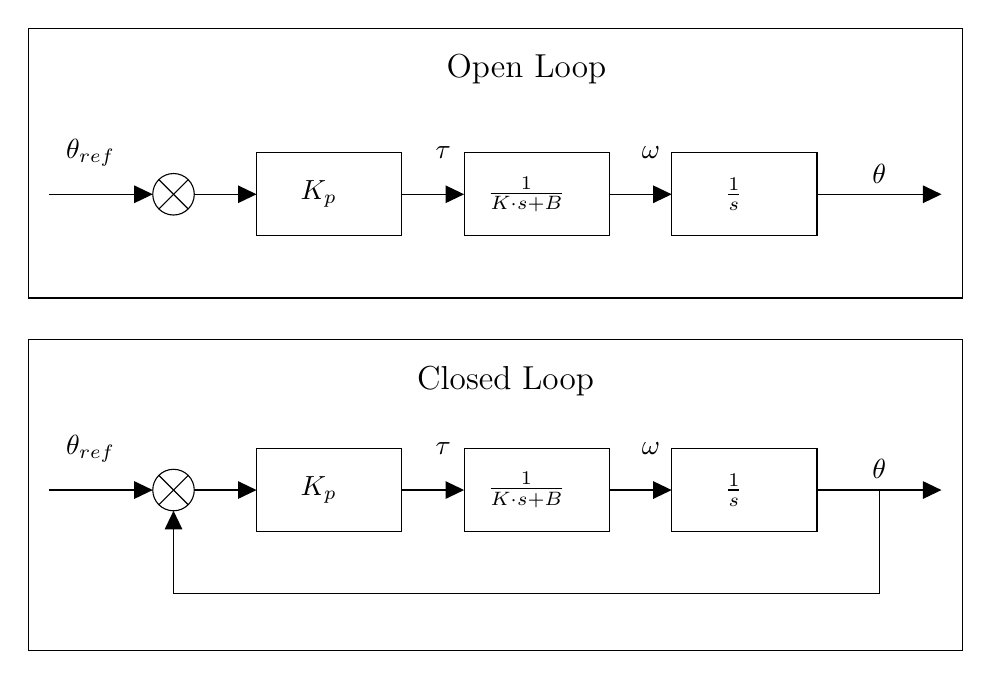
\begin{tikzpicture}[x=0.75pt,y=0.75pt,yscale=-1,xscale=1]
%uncomment if require: \path (0,328.50892877578735); %set diagram left start at 0, and has height of 328.50892877578735

%Shape: Rectangle [id:dp12482796861282974] 
\draw   (140,80) -- (210,80) -- (210,120) -- (140,120) -- cycle ;
%Straight Lines [id:da5706724332227189] 
\draw    (40,100) -- (88,100) ;
\draw [shift={(90,100)}, rotate = 180] [fill={rgb, 255:red, 0; green, 0; blue, 0 }  ][line width=0.75]  [draw opacity=0] (8.93,-4.29) -- (0,0) -- (8.93,4.29) -- cycle    ;

%Flowchart: Summing Junction [id:dp53704430353601] 
\draw   (90,100) .. controls (90,94.48) and (94.48,90) .. (100,90) .. controls (105.52,90) and (110,94.48) .. (110,100) .. controls (110,105.52) and (105.52,110) .. (100,110) .. controls (94.48,110) and (90,105.52) .. (90,100) -- cycle ; \draw   (92.93,92.93) -- (107.07,107.07) ; \draw   (107.07,92.93) -- (92.93,107.07) ;
%Straight Lines [id:da3178828171562029] 
\draw    (110,100) -- (138,100) ;
\draw [shift={(140,100)}, rotate = 180] [fill={rgb, 255:red, 0; green, 0; blue, 0 }  ][line width=0.75]  [draw opacity=0] (8.93,-4.29) -- (0,0) -- (8.93,4.29) -- cycle    ;

%Shape: Rectangle [id:dp28027349651381117] 
\draw   (240,80) -- (310,80) -- (310,120) -- (240,120) -- cycle ;
%Straight Lines [id:da11899224305491352] 
\draw    (210,100) -- (238,100) ;
\draw [shift={(240,100)}, rotate = 180] [fill={rgb, 255:red, 0; green, 0; blue, 0 }  ][line width=0.75]  [draw opacity=0] (8.93,-4.29) -- (0,0) -- (8.93,4.29) -- cycle    ;

%Shape: Rectangle [id:dp31656367205122615] 
\draw   (340,80) -- (410,80) -- (410,120) -- (340,120) -- cycle ;
%Straight Lines [id:da5367106543687827] 
\draw    (310,100) -- (338,100) ;
\draw [shift={(340,100)}, rotate = 180] [fill={rgb, 255:red, 0; green, 0; blue, 0 }  ][line width=0.75]  [draw opacity=0] (8.93,-4.29) -- (0,0) -- (8.93,4.29) -- cycle    ;

%Straight Lines [id:da7913281226659683] 
\draw    (410,100) -- (468,100) ;
\draw [shift={(470,100)}, rotate = 180] [fill={rgb, 255:red, 0; green, 0; blue, 0 }  ][line width=0.75]  [draw opacity=0] (8.93,-4.29) -- (0,0) -- (8.93,4.29) -- cycle    ;

%Shape: Rectangle [id:dp11142722632197088] 
\draw   (30,20) -- (480,20) -- (480,150) -- (30,150) -- cycle ;
%Shape: Rectangle [id:dp14600397799019293] 
\draw   (140,222.5) -- (210,222.5) -- (210,262.5) -- (140,262.5) -- cycle ;
%Straight Lines [id:da4243355948071521] 
\draw    (40,242.5) -- (88,242.5) ;
\draw [shift={(90,242.5)}, rotate = 180] [fill={rgb, 255:red, 0; green, 0; blue, 0 }  ][line width=0.75]  [draw opacity=0] (8.93,-4.29) -- (0,0) -- (8.93,4.29) -- cycle    ;

%Flowchart: Summing Junction [id:dp6729381602093008] 
\draw   (90,242.5) .. controls (90,236.98) and (94.48,232.5) .. (100,232.5) .. controls (105.52,232.5) and (110,236.98) .. (110,242.5) .. controls (110,248.02) and (105.52,252.5) .. (100,252.5) .. controls (94.48,252.5) and (90,248.02) .. (90,242.5) -- cycle ; \draw   (92.93,235.43) -- (107.07,249.57) ; \draw   (107.07,235.43) -- (92.93,249.57) ;
%Straight Lines [id:da14869215035902505] 
\draw    (110,242.5) -- (138,242.5) ;
\draw [shift={(140,242.5)}, rotate = 180] [fill={rgb, 255:red, 0; green, 0; blue, 0 }  ][line width=0.75]  [draw opacity=0] (8.93,-4.29) -- (0,0) -- (8.93,4.29) -- cycle    ;

%Shape: Rectangle [id:dp9900763090446374] 
\draw   (240,222.5) -- (310,222.5) -- (310,262.5) -- (240,262.5) -- cycle ;
%Straight Lines [id:da7760938350165698] 
\draw    (210,242.5) -- (238,242.5) ;
\draw [shift={(240,242.5)}, rotate = 180] [fill={rgb, 255:red, 0; green, 0; blue, 0 }  ][line width=0.75]  [draw opacity=0] (8.93,-4.29) -- (0,0) -- (8.93,4.29) -- cycle    ;

%Shape: Rectangle [id:dp19026495853512104] 
\draw   (340,222.5) -- (410,222.5) -- (410,262.5) -- (340,262.5) -- cycle ;
%Straight Lines [id:da42905616589605233] 
\draw    (310,242.5) -- (338,242.5) ;
\draw [shift={(340,242.5)}, rotate = 180] [fill={rgb, 255:red, 0; green, 0; blue, 0 }  ][line width=0.75]  [draw opacity=0] (8.93,-4.29) -- (0,0) -- (8.93,4.29) -- cycle    ;

%Straight Lines [id:da668486289799261] 
\draw    (410,242.5) -- (468,242.5) ;
\draw [shift={(470,242.5)}, rotate = 180] [fill={rgb, 255:red, 0; green, 0; blue, 0 }  ][line width=0.75]  [draw opacity=0] (8.93,-4.29) -- (0,0) -- (8.93,4.29) -- cycle    ;

%Straight Lines [id:da5740200387655516] 
\draw    (100,254.5) -- (100,292.5) ;

\draw [shift={(100,252.5)}, rotate = 90] [fill={rgb, 255:red, 0; green, 0; blue, 0 }  ][line width=0.75]  [draw opacity=0] (8.93,-4.29) -- (0,0) -- (8.93,4.29) -- cycle    ;
%Straight Lines [id:da1492709801617349] 
\draw    (100,292.5) -- (440,292.5) ;


%Straight Lines [id:da5671703763154259] 
\draw    (440,242.5) -- (440,292.5) ;


%Shape: Rectangle [id:dp043811444149466805] 
\draw   (30,170) -- (480,170) -- (480,320) -- (30,320) -- cycle ;

% Text Node
\draw (60,80) node   {$\theta _{ref}$};
% Text Node
\draw (170,100) node   {$K_{p}$};
% Text Node
\draw (230,80) node   {$\tau $};
% Text Node
\draw (270,100) node   {$\frac{1}{K\cdot s+B}$};
% Text Node
\draw (370,100) node   {$\frac{1}{s}$};
% Text Node
\draw (330,80) node   {$\omega $};
% Text Node
\draw (440,90) node   {$\theta $};
% Text Node
\draw (270,40) node  [align=left] {{\large Open Loop}};
% Text Node
\draw (60,222.5) node   {$\theta _{ref}$};
% Text Node
\draw (170,242.5) node   {$K_{p}$};
% Text Node
\draw (230,222.5) node   {$\tau $};
% Text Node
\draw (270,242.5) node   {$\frac{1}{K\cdot s+B}$};
% Text Node
\draw (370,242.5) node   {$\frac{1}{s}$};
% Text Node
\draw (330,222.5) node   {$\omega $};
% Text Node
\draw (440,232.5) node   {$\theta $};
% Text Node
\draw (260,190) node  [align=left] {{\large Closed Loop}};


\end{tikzpicture}

    \caption{Open- and closed loop are control schemes and that show how the signal runs through a controller}
    \label{fig:openclose}
\end{figure}